\documentclass[a4paper, twoside, 11pt, spanish]{book}

%% Paquetes
\usepackage[es-tabla]{babel}
\usepackage{amsmath, amsfonts, amssymb, amsthm}
\usepackage{color, graphicx, rotating, subcaption}
\usepackage[margin=2.2cm]{geometry}
\usepackage{hyperref, url}
\usepackage[font=small, labelfont=bf]{caption}
\usepackage{enumerate, enumitem}
\usepackage{tabularx}
\usepackage{ctable}
\usepackage{multicol}

\usepackage[square,numbers,sort&compress]{natbib}

\renewcommand{\baselinestretch}{1.2} % interlineado
\decimalpoint{} % cambia coma por punto

\DeclareMathOperator*{\argmax}{arg\,max}
\DeclareMathOperator*{\argmin}{arg\,min}

\theoremstyle{definition}
\newtheorem{theorem}{Teorema}[chapter]
\newtheorem{lemma}[theorem]{Lema}
\newtheorem{corollary}[theorem]{Corolario}
\newtheorem{remark}{Observaci\'on}[chapter]
\newtheorem{definition}{Definici\'on}[chapter]
\newtheorem{remarkex}{Observaci\'on}[chapter]


%% Bibliografia
\bibliographystyle{unsrtnat}
\addto{\captionsspanish}{\renewcommand{\bibname}{Referencias}}

%% Tablas
\renewcommand{\tablename}{Tabla}
\renewcommand{\contentsname}{Índice}

% Encabezados y pies de pagina solo con numero de pagina
\pagestyle{plain}

\begin{document}
 
\frontmatter

% Caratula
\newgeometry{top=5cm,bottom=2cm,left=3cm,right=3cm}
%%
%% Caratula de la tesis
%%
\thispagestyle{empty}

\begin{center}
  
\includegraphics[scale = 0.3]{logofac.jpg}
  
  \medskip
  UNIVERSIDAD DE BUENOS AIRES
  
  Facultad de Ciencias Exactas y Naturales
  
 
  
  \vspace{3cm}
  \textbf{\large Estimación por intervalos de las proporciones de clases en muestras sin etiquetar utilizando la distribución Poisson-Binomial}
  
  \vspace{2cm}
  Tesis presentada para optar al título de Magister en Estadística Matemática de
  la Universidad de Buenos Aires
  
  \vspace{2cm}
  \textbf{Ing. Maximiliano Marufo da Silva}
\end{center}


\vspace{1.5cm}
\noindent Director de tesis: Dr.~Andrés Farall
 

\vspace{1cm}
\noindent Buenos Aires,  2023.


\cleardoublepage{}

% INDICE
\tableofcontents 

% Restauro los margenes originales
\restoregeometry{}

% CUERPO PRINCIPAL
\mainmatter{}

\renewcommand{\baselinestretch}{1.5} % interlineado

\chapter{Introducción}

\section{Marco teórico}

La tarea de cuantificación (conocida en inglés como {\it quantification\/})
consiste en proporcionar predicciones agregadas o resumen para conjuntos de
datos en vez predicciones particulares sobre los datos individuales (por
ejemplo, para el caso de clasificación, predecir la proporción de clases de un
conjunto en vez de la clase de cada individuo), aplicando un modelo que se
ajuste usando datos de entrenamiento cuya distribución puede ser distinta a la
de los datos de prueba~\cite{forman2005counting}.

Si bien en principio no es necesario realizar predicciones por cada individuo,
muchos de los métodos se basan en obtener la cuantificación de esa manera, ya
que hacer predicciones individuales suele ser un requisito de por sí de las
aplicaciones prácticas, o porque ya existen en ellas sistemas que las generen.
Además, cabe aclarar que si bien la aplicación más popular es con respecto a
tareas de clasificación (sobre las cuales basaremos este trabajo, y en
particular, sobre clasificación binaria), también se puede aplicar
cuantificación a problemas de regresión, ordinalidad, etc.

Un ejemplo práctico puede ser predecir la proporción de comentarios a favor o en
contra sobre un producto, servicio o candidato en una red social. En este caso,
se puede utilizar un clasificador para predecir por cada comentario si la
opinión es positiva (o negativa), y luego obtener la proporción de comentarios a
favor contándolos y dividiéndolos por el total (este método es el más simple y
es conocido como {\it Classify \& Count\/} o {\it CC\/}).

Si hablamos entonces de cuantificación binaria, se tiene que por cada muestra $i
\in \{1,\dots,n\}$, $(\mathbf{X}_i,Y_i,S_i)$ es un vector de variables
aleatorias tal que $\mathbf{X}_i \in \mathbb{R}^d$ son las características de la
muestra, $Y_i \in \{1,0\}$ indica la clase a la que pertenece y $S_i \in
\{1,0\}$ indica si fue etiquetada (y pertenece entonces al conjunto de
entrenamiento) o no. Es decir, cuando $S_i=0$, entonces $Y_i$ no es observable.
En la cuantificación binaria, se desea estimar $\theta:= \mathbb{P}(Y=1|S=0)$,
es decir, la prevalencia de etiquetas positivas entre muestras no etiquetadas.
Esta prevalencia no se asume de ser la misma que en las muestras etiquetadas,
$\mathbb{P}(Y=1|S=1)$. Además, el estimador de $\theta$ debe depender sólo de
los datos disponibles, es decir, de las características de todas las muestras y
de las etiquetas que fueron obtenidas. Los supuestos que se asumen
son~\cite{vaz2019quantification}:

\begin{itemize}
  \item $(\mathbf{X}_1,Y_1,S_1) \dots (\mathbf{X}_n,Y_n,S_n)$ son independientes
  \item Por cada $s \in \{0,1\}$,
  $(\mathbf{X}_1,Y_1)|S_1=s,\dots,(\mathbf{X}_n,Y_n)|S_n=s$ son idénticamente
  distribuidas.
  \item Por cada $(y_1,\dots,y_n)\in{\{0,1\}}^n$,
  $(\mathbf{X}_1,\dots,\mathbf{X}_n)$ es independiente de $(S_1,\dots,S_n)$
  condicionado a $(Y_1,\dots,Y_n)=(y_1,\dots,y_n)$ 
\end{itemize}

Si bien existen varios métodos propuestos para el aprendizaje de
cuantificación~\cite{esuli2023learning, gonzalez2017review}, el mismo es todavía
relativamente desconocido incluso para expertos en aprendizaje automático. La
razón principal es la creencia errónea de que es una tarea trivial que se puede
resolver usando un método directo, como {\it CC}. La cuantificación requiere
métodos más sofisticados si el objetivo es obtener modelos óptimos, y su
principal dificultad radica en la definición del problema, ya que las
distribuciones de los datos de entrenamiento y de prueba pueden ser distintas.
Por ejemplo, si la diferencia entre $\mathbb{P}(Y=1|S=0)$ y
$\mathbb{P}(Y=1|S=1)$ es grande, los métodos simples como {\it CC\/} suelen
tener bajo rendimiento.

Un método de cuantificación muy popular en la literatura y que sí se adapta a
los cambios entre $\mathbb{P}(Y=1|S=0)$ y $\mathbb{P}(Y=1|S=1)$ es el propuesto
por~\citet{saerens2002adjusting}, conocido como {\it Expectation Maximization
for Quantification\/} -{\it EMQ\/}- o {\it SLD\/} por las siglas de sus autores.
El mismo es un método iterativo que corrige, mediante el Teorema de Bayes, las
predicciones de probabilidad de pertenencia a las clases dadas por el modelo de
clasificación ya ajustado (sin necesidad de reajuste), y como consecuencia
estima también la proporción de clases en la muestra de prueba. Este método es
una aplicación directa del algoritmo de Esperanza-Maximización {\it -EM-}, y se
puede probar que maximiza la verosimilitud en los datos de prueba. Se ha
estudiado también que el método {\it EMQ\/} mejora aún más las predicciones de
cuantificación si el clasificador utilizado está
calibrado~\cite{esuli2020critical, alexandari2020maximum}, es decir, si sus
predicciones de probabilidad asociadas a las clases predichas representan la
probabilidad real de pertenencia a las clases~\cite{guo2017calibration}.

Por otro lado, muy pocos son los trabajos sobre la construcción de intervalos de
confianza y predicción en cuantificación~\cite{tasche2019confidence}. La mayoría
de ellos se basan en emplear los métodos de predicción puntual junto con la
técnica de {\it bootstrapping\/}~\cite{hopkins2010method,
daughton2020constructing, daughton2021bootstrapping}, que puede ser
computacionalmente costosa en este tipo de tareas, o en métodos
asintóticos~\cite{vaz2019quantification}, que no funcionan bien con tamaños de
muestra pequeños y además requieren estimar la varianza. Dentro de los trabajos
sobre intervalos de confianza o predicción en cuantificación aplicada a la
clasificación (no se encontraron de hecho trabajos sobre intervalos en otro tipo
de problemas), Keith y O'Connor~\cite{keith2018uncertainty} proponen dos
métodos:

\begin{itemize}
    \item El {\it baseline}, al que llaman {\it PB-PCC}, es un método asintótico
    basado en la distribución Poisson-Binomial~\cite{le1960approximation,
    wang1993number}, donde proponen utilizar la media y varianza conocida para
    esta distribución para calcular el intervalo mediante la distribución
    normal. Existen tres problemas en el método propuesto en el trabajo:
        \begin{enumerate}
            \item Se basa en el método de cuantificación de predicción puntual
            conocido como {\it Probabilistic Classify \& Count -PCC-}, que no
            suele tener muy buenos resultados ya que no se ajusta a las
            diferencias entre $\mathbb{P}(Y=1|S=0)$ y
            $\mathbb{P}(Y=1|S=1)$.\label{keith_item_uno}
            \item En el trabajo no se verifica que el clasificador esté
            calibrado, lo que podría degradar los resultados del
            cuantificador.\label{keith_item_dos}
            \item Los métodos asintóticos no son buenos con muestras pequeñas.
        \end{enumerate}
    \item Su propuesta de mejora se basa en computar la verosimilitud marginal
    sobre $\theta$, la proporción de clases en la población de prueba, para
    obtener la distribución {\it a posteriori\/} de $\theta$. Luego, para
    obtener la predicción puntual se obtiene el máximo de la distribución. Es
    decir, que al igual que el método {\it EMQ}, se busca maximizar la
    verosimilitud, pero en este caso sin utilizar el algoritmo {\it EM\/} sino
    de forma directa. Para obtener en cambio los intervalos, se proponen dos
    opciones, la primera es usar la aproximación asintótica y la segunda es
    construir una grilla para la distribución {\it a posteriori\/} de $\theta$.
    Este método es bastante efectivo. Sin embargo, hay que tener en cuenta que
    aquí se estima la proporción de clases en la población de prueba, y no en la
    muestra de prueba.
\end{itemize}

~\citet{denham2021gain} propone un método que asume condiciones más generales de
cambio en las distribuciones entre los datos de entrenamiento y de prueba, ya
que no asume la tercera suposición mencionada anteriormente. El método que
proponen tiene, sin embargo, peor desempeño cuando esa condición sí se cumple.
No obstante, es interesante resaltar los dos métodos {\it baseline\/} que
utilizan para comparar con su propuesta de mejora:

\begin{itemize}
    \item El primer {\it baseline\/} es también basado en {\it PB-PCC\/} y
    similar al propuesto en Keith y O'Connor. La diferencia en este trabajo es
    que en vez de usar la aproximación asintótica, computan la función de
    distribución exacta mediante el método propuesto
    por~\citet{hong2013computing}, que utiliza la transformada rápida de Fourier
    ({\it FFT\/}) para hacerlo de forma eficiente. Este método sigue teniendo
    los primeros dos problemas mencionados en~\ref{keith_item_uno}
    y~\ref{keith_item_dos}.
    \item El segundo {\it baseline\/} es muy similar a la propuesta de mejora de
    Keith y O'Connor. La única diferencia es que usa el algoritmo de {\it EM\/}
    en vez de hacer el cálculo directo para obtener el máximo de la distribución
    {\it a posteriori}.
\end{itemize}

\section{Propuesta}

Se propone un método para la elaboración de intervalos de predicción de la
proporción de clases en muestras de prueba sin etiquetar, a partir de un
conjunto de datos con etiquetas conocidas (conjunto de entrenamiento). Los pasos
son:

\begin{enumerate}
    \item Ajustar un modelo de clasificación con los datos de entrenamiento
    \item Aplicar un método de calibración al clasificador para crear buenos
    estimadores de probabilidad para cada individuo.
        \begin{itemize}
            \item Se compararon todos los métodos de calibración mencionados en
            la bibliografía, evaluados bajo el problema de cuantificación,
            obteniendo los mejores resultados con los métodos propuestos
            en~\citet{alexandari2020maximum}.
        \end{itemize}
    \item Aplicar el método de cuantificación de estimación puntual de
    preferencia.\label{propuesta_item_tres}
        \begin{itemize}
            \item Se compararon los principales métodos mencionados en la
            bibliografía, obteniendo los mejores resultados con los métodos de
            {\it EMQ\/} y {\it PACC}.
        \end{itemize}
    \item Aplicar el paso de maximización de la esperanza propuesto
    en~\citet{saerens2002adjusting} para ajustar las predicciones de
    probabilidad de cada individuo en base a la predicción puntual de la
    proporción de clases obtenidas con el método elegido
    en~\ref{propuesta_item_tres}.
    \item Aplicar el método propuesto por~\citet{hong2013computing} para obtener
    la distribución exacta de la proporción de clases en la muestra de
    prueba.\label{propuesta_item_cinco}
    \item Utilizar la distribución obtenida en~\ref{propuesta_item_cinco} para
    elaborar un intervalo de predicción exacto de la proporción de clases en la
    muestra con el nivel que corresponda.
\end{enumerate}

Se presenta el método tanto de forma teórica como su evaluación empírica. Se
elaboraron simulaciones para su evaluación y comparación con los métodos
propuestos en Keith y O'Connor~\cite{keith2018uncertainty},
en~\citet{denham2021gain} y con los intervalos obtenidos mediante {\it
bootstrapping}.

\chapter{Problema}\label{problema}

\section{Introducción}\label{problema:introduccion}

En algunas aplicaciones vinculadas a la clasificación, el objetivo final no es
determinar a qué clase (o clases) pertenece cada una de las instancias
individuales de un conjunto de datos no etiquetado, sino estimar la proporción
(tambíen llamada `prevalencia', `frecuencia relativa' o `probabilidad prior') de
cada clase en los datos sin etiquetar. En los últimos años se ha señalado que,
en estos casos, tiene sentido optimizar directamente algoritmos de aprendizaje
automático para este objetivo, en lugar de simplemente optimizar clasificadores
para etiquetar instancias individuales.

La tarea de ajustar estimadores de prevalencia de clases a través del
aprendizaje supervisado se conoce como `aprender a cuantificar' o, más
simplemente, cuantificar o {\it quantification\/} (término acuñado
por~\citet{forman2005counting}, quien planteó el problema por primera vez). Se
sabe que cuantificar mediante la clasificación de cada instancia sin etiquetar a
través de un clasificador estándar y luego contando las instancias que han sido
asignadas a cada clase (el método {\it Classify \& Count\/}) generalmente
conduce a estimadores de prevalencia de clases sesgados, es decir, obtienen poca
exactitud en la cuantificación. Como resultado, se han desarrollado métodos que
abordan la cuantificación como una tarea en sí.

Para ver la importancia de diferenciar el problema de cuantificación del de
clasificación, veamos dos ejemplos. En el primero, una empresa que ofrece un
servicio a sus clientes realiza una encuesta con varias preguntas para
determinar el grado de satisfacción de cada persona. El objetivo de le empresa
es determinar aquellos clientes que podrían no estar conformes con el servicio y
ofrecerles una mejora en las condiciones para retenerlos. En el segundo ejemplo,
una consultora analiza tweets para estimar el grado de aprobación de candidatos
políticos. Aquí, la consultora no está interesado en predecir si un individuo
específico está a favor o en contra, sino en cuántos encuestados, del número
total de encuestados, aprueban al candidato, es decir, en conocer la prevalencia
de la clase positiva.

Mientras en el primer escenario el interés es a nivel individual, en el último,
el nivel agregado es lo que importa; en otras palabras, en el primer escenario
la clasificación es el objetivo, mientras que en el segundo el verdadero
objetivo es la cuantificación. De hecho, en la mayoría de las aplicaciones las
predicciones que interesan no son a nivel individual sino a nivel colectivo;
ejemplos de tales campos son la investigación de mercado, la ciencia política,
las ciencias sociales, modelado ecológico y epidemiología.

\begin{figure}[h]
    \centering
    \begin{subfigure}[t]{0.4\textwidth}
        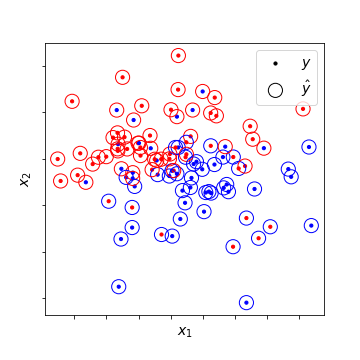
\includegraphics[width=\textwidth]{../plots_teoria/intro_scatterplot.png}
        \caption{Clasificación}
    \end{subfigure}
    \hfill
    \begin{subfigure}[t]{0.4\textwidth}
        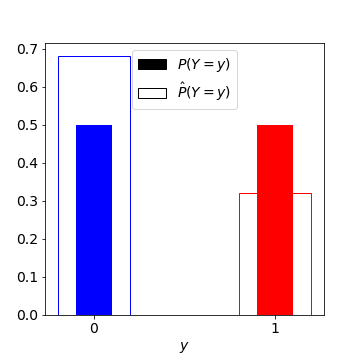
\includegraphics[width=\textwidth]{../plots_teoria/intro_barplot.png}
        \caption{Cuantificación}
    \end{subfigure}
    \caption{En la clasificación, la predicción es a nivel individual, mientras
    que en la cuantificación es a nivel agregado.}\label{fig:intro}
\end{figure}

En resumen, y generalizando no sólo para clasificación sino también a otros
problemas (regresión, ordinalidad, etc), la tarea de cuantificación consiste en
proporcionar predicciones agregadas para conjuntos de datos, en vez de
predicciones particulares sobre los datos individuales. Si bien en principio no
es necesario realizar predicciones por cada individuo, muchos de los métodos se
basan en obtener la cuantificación de esa manera, ya que hacer predicciones
individuales suele ser un requisito de por sí de las aplicaciones prácticas, o
porque ya existen en ellas modelos que las generen.

La literatura sobre métodos relacionados con cuantificación está un tanto
desconectada. Algunos de los métodos que pueden usarse como cuantificadores han
sido ideados para otros fines, principalmente para mejorar la precisión en
clasificación cuando cambia el dominio. El desempeño de este último grupo ha
sido normalmente estudiado solo en términos de mejora en las tareas de
clasificación pero no como cuantificadores. Dado este escenario, y debido a la
variedad de campos en los que ha surgido como una necesidad de aplicación, los
algoritmos que se pueden aplicar para tareas de cuantificación aparecen en
artículos que usan diferentes palabras clave y nombres, como {\it
counting\/}~\cite{lewis1995evaluating}, {\it prior probability
shift\/}~\cite{moreno2012unifying, storkey2009training}, {\it posterior
probability estimation\/}~\cite{alaiz2011class}, {\it class prior
estimation\/}~\cite{du2014class, chan2006estimating, zhang2010transfer}, {\it
class prior change\/}~\cite{du2014semi}, {\it prevalence
estimation\/}~\cite{barranquero2013study}, {\it class ratio
estimation\/}~\cite{asoh2012fast} o {\it class distribution
estimation\/}~\cite{gonzalez2013class, limsetto2011handling,
xue2009quantification}, por citar solo algunos de ellos.

\section{Tipos de Cuantificación}\label{problema:tipos}

Aunque el estudio de la cuantificación se ha centrado principalmente en el
dominio de clasificación, la cuantificación también aparece en otros tipos de
problemas de aprendizaje automático, como la regresión, la clasificación
ordinal, el aprendizaje sensible al costo y la cuantificación en redes.

De manera similar a la regresión, aprender a cuantificar admite diferentes
problemas de interés aplicativo, basados en cuántas clases distintas existen en
el problema, y en cuántas de las clases se pueden atribuir al mismo tiempo al
mismo individuo. Así, los problemas de cuantificación se dividen de esta manera:

\begin{enumerate}
    \item Etiquetado simple {\it (Single-Label Quantification -SLQ-)\/}: cuando
    cada individuo pertenece exactamente a una de las clases en
    $C=\{c_1,\dots,c_{\#C}\}$.
    \item Etiquetado múltiple {\it (Multi-Label Quantification -MLQ-)\/}: cuando
    cada individuo puede pertenecer a cualquier número de clases (cero, una o
    varias) en $C=\{c_1,\dots,c_{\#C}\}$.
    \item Cuantificación Binaria {\it (Binary Quantification -BQ-)\/}:
    \begin{enumerate}
        \item en {\it SLQ\/} con $\#C=2$, (en este caso $C=\{c_1,c_2\}$, y cada
        individuo pertenece a $c_1$ o $c_2$)
        \item en {\it MLQ\/} con $\#C=1$, (en este caso $C=\{c\}$, y cada
        individuo pertenece o no a $c$)
    \end{enumerate}
    \item Cuantificación Ordinal {\it (Ordinal Quantification -OQ-)\/}: cuando
    existe un orden $c_1 \prec \dots \prec c_{\#C}$ en
    $C=\{c_1,\dots,c_{\#C}\}$.
    \item Cuantificación de Regresión {\it (Regression Quantification -RQ-)\/}:
    cuando no hay un conjunto de clases involucradas, sino que cada individuo
    está etiquetado con una puntuación de valor real y la cuantificación
    equivale a estimar la fracción de ítems cuya puntuación está en un intervalo
    dado $[a, b]$ con ${a, b \in \mathbb{R}^d}$.
\end{enumerate}

\section{Marco teórico}\label{problema:marco_teorico}

Si hablamos entonces de cuantificación binaria, se tiene que por cada muestra $i
\in \{1,\dots,n\}$, $(\boldsymbol{X}_i,Y_i,S_i)$ es un vector de variables
aleatorias tal que $\boldsymbol{X}_i \in \mathbb{R}^d$ son las características
de la muestra, $Y_i \in C$ con $C=\{1,0\}$ indica la clase a la que pertenece y
$S_i \in \{1,0\}$ indica si fue etiquetada (y pertenece entonces al conjunto de
entrenamiento) o no. Es decir, cuando $S_i=0$, entonces $Y_i$ no es observable.
El objectivo es estimar $\theta:= \mathbb{P}(Y=1|S=0)$\footnote{En
cuantificación, se lo nombra generalmente como $p$ (o $p_1,\dots,p_{\#C}$ o
$p(c)$ para el caso multiclase) en vez de $\theta$, por lo que en este trabajo
también se usará esta nomenclatura.}, es decir, la prevalencia de etiquetas
positivas entre muestras no etiquetadas. Esta prevalencia no se asume de ser la
misma que en las muestras etiquetadas, $\mathbb{P}(Y=1|S=1)$. Además, el
estimador de $\theta$ debe depender sólo de los datos disponibles, es decir, de
las características de todas las muestras y de las etiquetas que fueron
obtenidas. Los supuestos que se asumen~\cite{vaz2019quantification} son:

\begin{itemize}
  \item $(\boldsymbol{X}_1,Y_1,S_1) \dots (\boldsymbol{X}_n,Y_n,S_n)$ son
  independientes
  \item Por cada $s \in \{0,1\}$,
  $(\boldsymbol{X}_1,Y_1)|S_1=s,\dots,(\boldsymbol{X}_n,Y_n)|S_n=s$ son
  idénticamente distribuidas.
  \item Por cada $(y_1,\dots,y_n)\in{\{0,1\}}^n$,
  $(\boldsymbol{X}_1,\dots,\boldsymbol{X}_n)$ es independiente de
  $(S_1,\dots,S_n)$ condicionado a $(Y_1,\dots,Y_n)=(y_1,\dots,y_n)$
\end{itemize}

Usando la distribución de probabilidad conjunta, podemos factorizar usando las
distribuciones condicionales:
\begin{equation}
    \mathbb{P}(\boldsymbol{X},Y,S)=\mathbb{P}(\boldsymbol{X}|Y,S)\mathbb{P}(Y|S)\mathbb{P}(S)
\end{equation}
Luego, usando el tercer supuesto mencionado, podemos
hacer~\cite{moreno2012unifying}:
\begin{equation}
    \mathbb{P}(\boldsymbol{X},Y,S)=\mathbb{P}(\boldsymbol{X}|Y)\mathbb{P}(Y|S)\mathbb{P}(S)
\end{equation}
Si bien existen varios métodos propuestos para el aprendizaje de
cuantificación~\cite{esuli2023learning, gonzalez2017review}, el mismo es todavía
relativamente desconocido incluso para expertos en aprendizaje automático. La
razón principal es la creencia errónea de que es una tarea trivial que se puede
resolver usando un método directo, como {\it CC}. La cuantificación requiere
métodos más sofisticados si el objetivo es obtener modelos óptimos, y su
principal dificultad radica en la definición del problema, ya que las
distribuciones de los datos de entrenamiento y de prueba pueden ser distintas.
Por ejemplo, si la diferencia entre $\mathbb{P}(Y=1|S=0)$ y
$\mathbb{P}(Y=1|S=1)$ es grande, los métodos simples como {\it CC\/} suelen
tener bajo rendimiento.


\section{Cambios en las distribuciones de los datos}\label{problema:cambios}

En lo últimos años ha habido un interés creciente en las aplicaciones que
presentan cambios en las distribuciones de datos (conocido en la blibliografía
por su término en inglés {\it dataset shift\/}). Estos problemas comparten el
hecho de que la distribución de los datos utilizados para entrenar es diferente
a la de los datos que se usan para predecir. Al igual que para el área de la
cuantificación, aquí también la literatura sobre el tema está dispersa y
diferentes autores usan diferentes nombres para referirse a los mismos
conceptos, o usan el mismo nombre para diferentes conceptos.

Teniendo en cuenta que en los problemas de clasificación tenemos:

\begin{itemize}
    \item Un conjunto de características o covariables $\boldsymbol{X}$.
    \item Una variable de respuesta $Y$.
    \item Una distribución de probabilidad conjunta
    $\mathbb{P}(Y=y,\boldsymbol{X=x})$.
\end{itemize}

La probabilidad conjunta $\mathbb{P}(Y,\boldsymbol{X})$ luego se puede escribir
como $\mathbb{P}(Y|\boldsymbol{X})\mathbb{P}(\boldsymbol{X})$ o como
$\mathbb{P}(\boldsymbol{X}|Y)\mathbb{P}(Y)$. Por otro lado, cuando usamos los
términos de entrenamiento ({\it train\/}) y prueba ({\it test\/}), nos referimos
a las datos disponibles para entrenar al clasificador y los datos presentes en
el entorno en el que se implementará el clasificador, respectivamente. Podemos
entonces también separar los datos en dos distribuciones distintas,
condicionando a la vaiable $S$ definida en~\ref{problema:marco_teorico}, siendo
$\mathbb{P}_{tr}(Y,\boldsymbol{X})=\mathbb{P}(Y,\boldsymbol{X}|S=1)$ y
$\mathbb{P}_{tst}(Y,\boldsymbol{X})=\mathbb{P}(Y,\boldsymbol{X}|S=0)$.

El {\it dataset shift\/} aparece cuando las distribuciones conjuntas de
entrenamiento y de prueba son diferentes, es decir, cuando
$\mathbb{P}_{tr}(Y,\boldsymbol{X}) \neq
\mathbb{P}_{tst}(Y,\boldsymbol{X})$.~\citet{moreno2012unifying} distingue las
distintas variantes del {\it dataset shift\/} según qué elementos mencionados
anteriormente cambian:

\begin{itemize}
    \item {\it Covariate shift}, cuando $\mathbb{P}_{tr}(Y|\boldsymbol{X}) =
    \mathbb{P}_{tst}(Y|\boldsymbol{X})$ y $\mathbb{P}_{tr}(\boldsymbol{X}) \neq
    \mathbb{P}_{tst}(\boldsymbol{X})$
    \item {\it Prior probability shift}, cuando
    $\mathbb{P}_{tr}(\boldsymbol{X}|Y) = \mathbb{P}_{tst}(\boldsymbol{X}|Y)$ y
    $\mathbb{P}_{tr}(Y) \neq \mathbb{P}_{tst}(Y)$
    \item {\it Concept shift}, cuando $\mathbb{P}_{tr}(Y|\boldsymbol{X}) \neq
    \mathbb{P}_{tst}(Y|\boldsymbol{X})$ y $\mathbb{P}_{tr}(\boldsymbol{X}) =
    \mathbb{P}_{tst}(\boldsymbol{X})$ o $\mathbb{P}_{tr}(\boldsymbol{X}|Y) \neq
    \mathbb{P}_{tst}(\boldsymbol{X}|Y)$ y $\mathbb{P}_{tr}(Y) =
    \mathbb{P}_{tst}(Y)$
\end{itemize}

Otros tipos de {\it dataset shift\/} surgen cuando
$\mathbb{P}_{tr}(Y|\boldsymbol{X}) \neq \mathbb{P}_{tst}(Y|\boldsymbol{X})$ y
$\mathbb{P}_{tr}(\boldsymbol{X}) \neq \mathbb{P}_{tst}(\boldsymbol{X})$ y cuando
$\mathbb{P}_{tr}(\boldsymbol{X}|Y) \neq \mathbb{P}_{tst}(\boldsymbol{X}|Y)$ y
$\mathbb{P}_{tr}(Y) \neq \mathbb{P}_{tst}(Y)$. Sin embargo, estos tipos de
cambios no se consideran generalmente en la literatura ya que aparecen mucho más
raramente, o incluso porque son dificiles o imposibles de resolver.

El problema de cuantificación se trata de un caso donde $\mathbb{P}_{tst}(Y)$ es
desconocido. Además, la mayoría de los métodos de cuantificación propuestos
asumen que $\mathbb{P}_{tr}(\boldsymbol{X}|Y) =
\mathbb{P}_{tst}(\boldsymbol{X}|Y)$, por lo que están dentro de los casos de
{\it prior probability shift}.

Por otro lado, en la mayoría de los casos el objetivo final de la implementación
es estimar algún parámetro de $\mathbb{P}_{tst}(Y)$. Por ejemplo, como ya
mencionamos anteriormente, en la cuantificación binaria, se desea estimar
$\theta:= \mathbb{P}(Y=1|S=0)$, o lo que es lo mismo, $p_{tst}:=
\mathbb{P}_{tst}(Y=1)$. Es decir, en la cuantificación la tarea indirectamente
suele ser aprender a aproximar una distribución desconocida (observando sólo
características de una muestra) mediante una distribución conocida. En
consecuencia, prácticamente todas las medidas de evaluación para la
cuantificación son divergencias, es decir, medidas de cómo una distribución
pronosticada difiere de la distribución real.

\begin{figure}[h]
    \centering
    \begin{subfigure}[t]{0.4\textwidth}
        \centering
        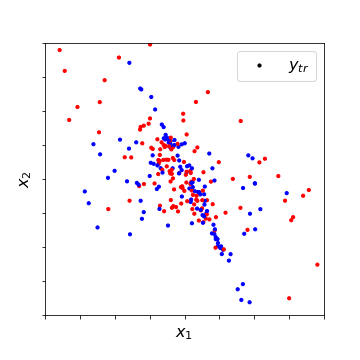
\includegraphics[width=\textwidth]{../plots_teoria/cambios_train_scatterplot.png}
        \caption{Muestra de entrenamiento}\label{cambios:datos_tr}
    \end{subfigure}
    \hfill
    \begin{subfigure}[t]{0.4\textwidth}
        \centering
        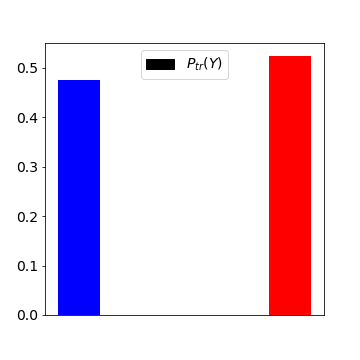
\includegraphics[width=\textwidth]{../plots_teoria/cambios_train_barplot.png}
        \caption{Prevalencia de clases en muestra de
        entrenamiento}\label{cambios:prevalencia_tr}
    \end{subfigure}
    \medskip
    \begin{subfigure}[t]{0.4\textwidth}
        \centering
        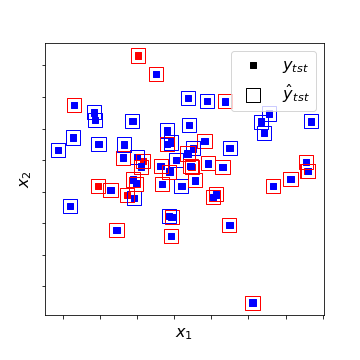
\includegraphics[width=\textwidth]{../plots_teoria/cambios_test_scatterplot.png}
        \caption{Clasificación en muestra de prueba. Para el modelo, las
        $y_{tst}$ son desconocidas.}\label{cambios:clasificacion_tst}
    \end{subfigure}
    \hfill
    \begin{subfigure}[t]{0.4\textwidth}
        \centering
        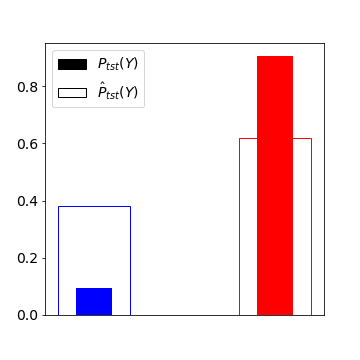
\includegraphics[width=\textwidth]{../plots_teoria/cambios_test_barplot.png}
        \caption{Prevalencia de clases verdadera y cuantificación en muestra de
        prueba}\label{cambios:cuantificacion_tst}
    \end{subfigure}
    \caption{El {\it prior probability shift\/} propio de los problemas de
    cuantificación puede hacer que los métodos simples de cuantificación, como
    {\it CC}, tengan grandes errores.}\label{fig:cambios}
\end{figure}

\section{El problema de clasificar y contar}\label{problema:clasificar_y_contar}

En ausencia de métodos para estimar los valores de prevalencia de clase de forma
directa, el primer método que suele pensarse para hacerlo es {\it Classify \&
Count}, es decir, clasificar cada individuo sin etiquetar y estimar los valores
de prevalencia de clase contando los individuos que fueron asignados a cada
clase. Sin embargo, esta estrategia es subóptima: si bien un clasificador
perfecto es también un cuantificador perfecto, un buen clasificador puede ser un
mal cuantificador. Para ver esto, se puede ver la definición de $F_1$, una
función de evaluación estándar para la clasificación binaria, que se define
como:
\begin{equation}
    F_1 = \frac{2 \cdot tp}{2 \cdot tp + fp + fn}
\end{equation}
donde $tp$, $fp$, $fn$ indican el número de verdaderos positivos, falsos
positivos y falsos negativos, respectivamente. Un buen clasificador puede ser un
mal cuantificador ya que $F_1$ considera buenos aquellos clasificadores que
mantienen la suma $fp + fn$ al mínimo; sin embargo, el objetivo de un algoritmo
de cuantificación debe ser mantener al mínimo $|fp-fn|$.

El análisis teórico de esta cuestión se basa en el supuesto de {\it prior
probability shift\/}~\ref{problema:cambios}. Bajo tal supuesto, la estimación
$\hat p$ obtenida por el enfoque {\it CC\/} depende sólo de las características
del clasificador, definido (para el caso binario) por su tasa de verdaderos
positivos ($tpr$), su tasa de falsos positivos ($fpr$) y de la prevalencia real
($p$):
\begin{equation}\label{ecuacion:tpr_fpr}
    \hat p(p) = p \cdot {tpr} + (1-p) \cdot {fpr}
\end{equation}
\begin{figure}[h]
    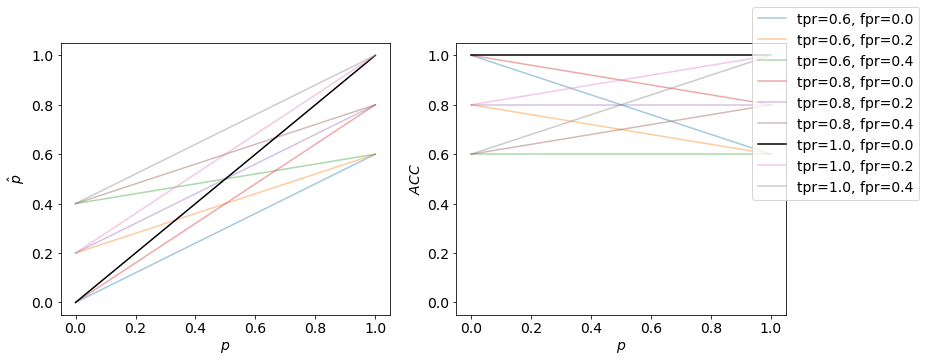
\includegraphics[width=\textwidth]{../plots_teoria/cc_tpr_fpr.png}
    \caption{La línea negra representa el cuantificador y clasificador perfecto,
    respectivamente. Las otras líneas muestran las estimaciones teóricas de
    $\hat p$ resultantes de aplicar la ecuación~\ref{ecuacion:tpr_fpr}, y el
    {\it accuracy\/} correspondiente al clasificador, según se varían los
    valores de $tpr$ y $fpr$}\label{fig:cc_tpr_fpr}
\end{figure}

El mal desempeño de {\it CC\/} fue demostrado mediante el siguiente teorema
por~\citet{forman2008quantifying}:

\begin{theorem}[Toerema de Forman]
    \citep[p.169]{forman2008quantifying}\label{teorema:forman} Para un
    clasificador imperfecto, el método {\it CC\/} subestimará la porporción
    verdadera de ejemplos positivos $p$ en un conjunto de prueba para $p>p^*$, y
    sobreestimará para $p<p^*$, donde $p^*$ es la proporción particular en la
    cual el método {\it CC\/} estima de forma correcta. Es decir, el método {\it
    CC\/} estima exactamente $p^*$ para un conjunto de prueba con $p^*$ muestras
    positivas.
\end{theorem}

La demostración (ver todos los detalles en~\citep[p.170]{forman2008quantifying})
supone que el cuantificador {\it CC\/} produce una predicción perfecta para una
prevalencia concreta, llamada $p^*$, y estudia su comportamiento cuando la
prevalencia cambia ligeramente. Suponiendo que $\hat p(p^*) = p^*$, cuando la
prevalencia cambia en una cantidad $\Delta \neq 0, p^* + \Delta$, la estimación
del método CC en tal caso será:
\begin{align}
\begin{split}
    \hat p(p^* + \Delta) &= (p^* + \Delta) \cdot {tpr} + (1-(p^* + \Delta)) \cdot {fpr} \\
    &= \hat p(p^*) + ({tpr} - {fpr}) \cdot \Delta \\
    &= p^* + ({tpr} - {fpr}) \cdot \Delta
\end{split}
\end{align}
La predicción del método {\it CC\/} será perfecta, $\hat p(p^* + \Delta) = (p^*
+ \Delta)$, sólo cuando el clasificador también es perfecto (${tpr} = 1$, ${fpr}
= 0$ y por tanto ${tpr} - {fpr} = 1$). Pero en el caso habitual, en el cual el
clasificador es imperfecto ($0 \leq {tpr} - \text {fpr} < 1$), cuando la
prevalencia aumenta ($\Delta > 0$), {\it CC\/} la subestima ($\hat p < p^* +
\Delta $), y cuando la prevalencia disminuye ($\Delta < 0$), {\it CC\/} la
sobreestima ($\hat p > p^* + \Delta $).

Un buen clasificador puede estar sesgado, es decir, puede mantener sus falsos
positivos al mínimo sólo a expensas de una cantidad sustancialmente mayor de
falsos negativos (o viceversa); si este es el caso, el clasificador es un mal
cuantificador. Este fenómeno no es infrecuente, especialmente en presencia de
datos desbalanceados. En tales casos, los algoritmos que minimizan las funciones
de pérdida de clasificacion ({\it Hamming}, {\it hinge}, etc) suelen generar
clasificadores con tendencia a elegir la clase mayoritaria, lo que implica un
número mucho mayor de falsos positivos que de falsos negativos para la clase
mayoritaria, lo que significa a su vez que tal algoritmo tenderá a subestimar
las clases minoritarias.

Los argumentos anteriores indican que no se debe considerar la cuantificación
como un mero subproducto de la clasificación, y debe estudiarse y resolverse
como una tarea en sí misma. Hay al menos otros dos argumentos que apoyan esta
idea. Uno es que las funciones que se utilizan para evaluar la clasificación no
se pueden utilizar para evaluar la cuantificación, ya que estas funciones miden,
en general, cuántos individuos han sido mal clasificados, y no cuánto difiere la
prevalencia de clase estimada del valor real. Esto significa que los algoritmos
que minimizan estas funciones están optimizados para la clasificación, y no para
la cuantificación. Un segundo argumento presentado por
~\citet{forman2008quantifying} es que los métodos diseñados específicamente para
cuantificar requieren menos datos de entrenamiento para alcanzar la misma
precisión de cuantificación que los métodos estándar basados en {\it CC}. Si
bien esta observación es de naturaleza empírica, también existen argumentos
teóricos que sustentan este hecho~\cite{vapnik1999overview}.

\section{Cuantificadores para la mejora de la
clasificación}\label{problema:mejora}

Debido a los problemas mencionados anteriormente de los clasificadores frente a
cambios en las distribuciones de los datos y frente a datos desbalanceados, los
algoritmos de cuantificación están cada vez más frecuentemente también siendo
usados en tareas que requieren predicciones individuales. Los mismos se emplean
como suplemento de clasificadores para suplir sus defectos frente a estos
problemas, ya que en algunos casos no sólo predicen los valores agregados, sino
que también mejoran las predicciones a nivel individual.

Por ejemplo, el {\it prior probability shift\/} puede hacer que los
clasificadores performen de manera subóptima. En el caso del clasificador óptimo
de Bayes, dado por:
\begin{equation}\label{ecuacion:bayes}
    h(\boldsymbol{x}) = \argmax_{y} p_{Y|\boldsymbol{X}=\boldsymbol{x}}(y) = \argmax_{y} \frac{p_{\boldsymbol{X}|Y=y}(\boldsymbol{x})p_Y(y)}{p_{\boldsymbol{X}}(\boldsymbol{x})}
\end{equation}
la decisión del clasificador depende de $p_Y(y)$, que es estimado con el dataset
de entrenamiento, siendo $\hat p_Y(y=1) = p_{tr}$. Es decir, que en caso de
$\mathbb{P}_{tr}(Y) \neq \mathbb{P}_{tst}(Y)$, la decisión final del
clasificador puede verse afectada negativamente. Para mejorar el rendimiento del
clasificador frente a estos casos, se debería usar $\hat p_Y(y=1) = p_{tst}$,
pero como $p_{tst}$ es generalmente desconocido, se puede usar un método de
cuantificación para estimarlo~\cite{saerens2002adjusting, alaiz2011class,
zhang2010transfer, xue2009quantification}.

\begin{figure}[H]
    \centerline{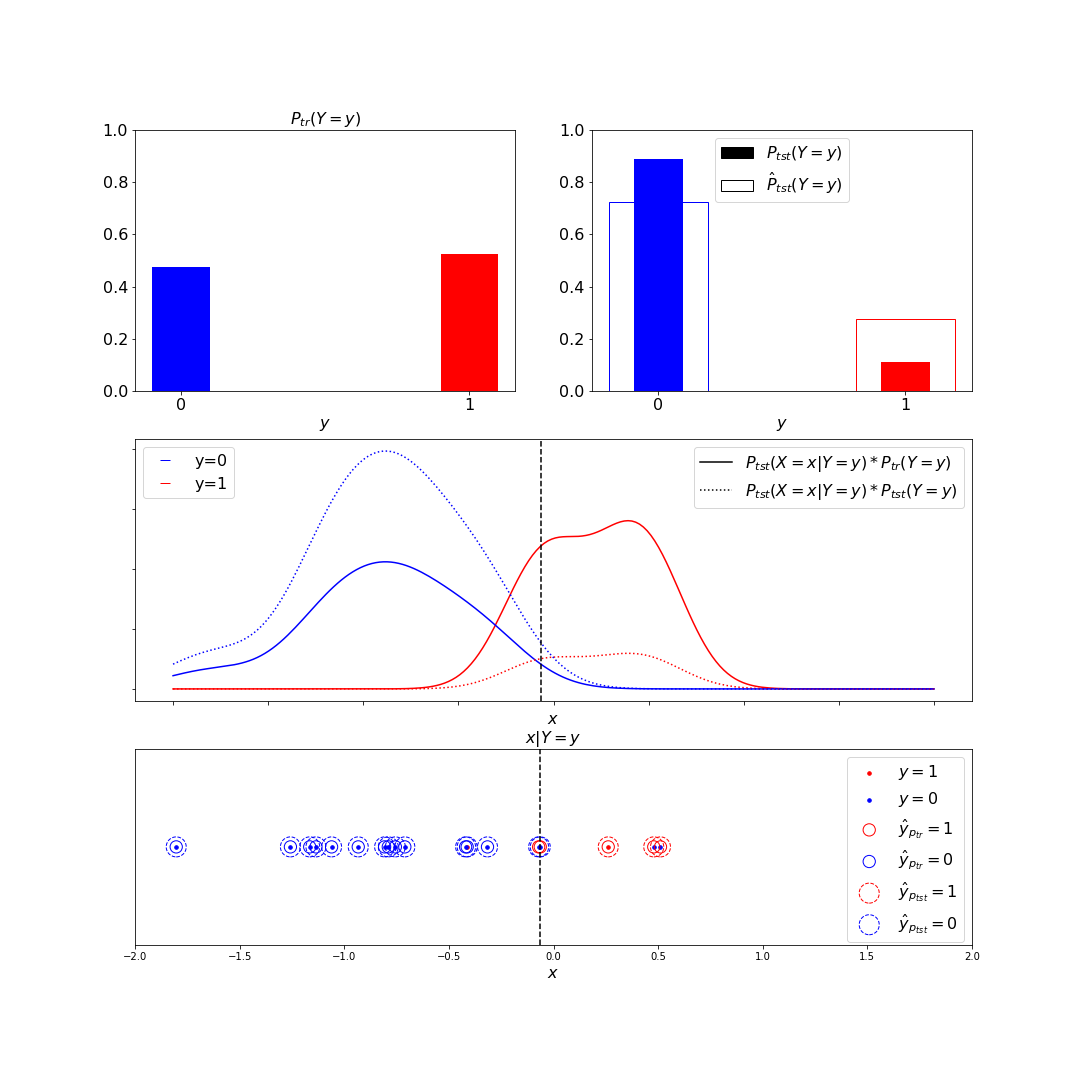
\includegraphics[width=0.75\textwidth]{../plots_teoria/bayes_classifier.png}}
    \caption{Ejemplo de como el {\it prior probability shift\/} puede alterar
    las predicciones del clasificador óptimo de Bayes. Vemos que si usaramos
    $\mathbb{P}_{tst}(Y)$ en vez de $\mathbb{P}_{tr}(Y)$, en este caso pasaría a
    predecir la clase azúl en vez de roja para toda
    $\boldsymbol{x}$.}\label{fig:bayes_classifier}
\end{figure}

Los métodos de cuantificación pueden usarse no sólo para mejorar el rendimiento
general de un clasificador, sino también para mejorar su equidad o {\it
fairness\/}~\cite{biswas2021ensuring}, es decir, su posibilidad de predecir
resultados independientes de un cierto conjunto de variables que consideramos
sensibles y no relacionadas con él (e.j.:~género, etnia, orientación sexual,
etc.). Por ejemplo, suponiendo que una variable $S$ debe considerarse sensible,
se puede estimar $\mathbb{P}_{tr}(Y|S)$. Luego, si los datos de entrenamiento
están sesgados, por ejemplo, con $\mathbb{P}_{tr}(Y=1|S=1) \gg
\mathbb{P}_{tr}(Y=1|S=0)$, pero se sabe que en las muestras a inferir esto no es
así, se puede optimizar el modelo de clasificación imponiento alguna penalidad
basada en la estimación de $\mathbb{P}_{tst}(Y|S)$, siendo esta última obtenido
por un cuantificador.

\chapter{Métodos de Evaluación}\label{evaluacion}

La evaluación de métodos de cuantificación es más compleja que en otros
problemas. En aprendizaje supervisado, típicamente se mide el rendimiento
estimando la probabilidad de predecir correctamente ejemplos individuales no
observados (sin condicionar -para la exactitud o {\it accuracy\/}- o
condicionando las probabilidades a las clases de pertenencia -para la
exhaustividad o {\it recall\/}- o predichas -para la precisión o {\it
precision\/}-). Sin embargo, en cuantificación, el rendimiento se evalúa para
conjuntos de datos. Esto implica que necesitamos una colección de muestras para
evaluar el rendimiento de un modelo. Dado un modelo $\overline{h}$, una función
de pérdida $L(\cdot, \cdot)$, y un conjunto de muestras de evaluación ${T_1,
\dots, T_s}$, el rendimiento de $\overline{h}$ es:

\begin{equation}
    Rendimiento(\overline{h}, L, {T_1, \dots , T_s}) = \frac{1}{s}
    \sum \limits_{j=1}^{s}L(\overline{h}, T_j)
    \label{ecuacion_rendimiento}
\end{equation}

Calcular la pérdida de un modelo sobre una muestra de prueba, $L(\overline{h},
T_j)$ no requiere de promediar sobre ejemplos individuales. Por ejemplo, en la
cuantificación binaria, sólo la prevalencia real $p$ y la prevalencia predicha
$\hat{p}$ se comparan por cada muestra.

En cuantificación, el problema de evaluación se relaciona con el cambio en la
distribución de datos entre la fase de entrenamiento y la de implementación del
modelo. Se requiere una colección de muestras de prueba variada y que represente
diversas distribuciones para evaluar correctamente el rendimiento del modelo y
evitar sesgos. Por esta razón, la mayoría de los experimentos reportados en la
literatura emplean conjuntos de datos tomados de otros problemas y se crean
conjuntos de prueba con cambios en las distribuciones creados artificialmente.
Este enfoque tiene la ventaja de que la cantidad del {\it dataset shift\/} se
puede controlar para estudiar el rendimiento de los modelos en diferentes
situaciones.

Las funciones de pérdida $L(\cdot, \cdot)$ serán elegidas de acuerdo al tipo de
problema y al objetivo particular de la aplicación. Como ya se mencionó, el
rendimiento de $\overline{h}$ será el promedio del resultado de la función de
pérdida por cada muestra de evaluación, de acuerdo a la
ecuación~\ref{ecuacion_rendimiento}. Se han propuesto en la literatura distintas
métricas de evaluación para problemas de {\it Single-Label Quantification
(SLQ)}. Estas también se pueden usar para {\it Binary Quantification (BQ)}, ya
que es un caso espacial del anterior, y para {\it Multi-Label Quantification},
ya que se pueden usar para cada $y \in C$. Esencialmente todas las medidas de
evaluación que se han propuesto son divergencias, es decir, medidas de cómo una
distribución difiere de otra. No se desarrollarán en esta tésis métricas para
{\it Ordinal Quantification\/} ni para {\it Regression Quantification }, ya que
no son útiles para nuestro objeto de estudio.

\section{Propiedades}\label{evaluacion:propiedades}

~\citet{sebastiani2020evaluation} define una serie de propiedades interesantes
para medidas de evaluación en {\it SLQ}. Un importante resultado de este
artículo es que ninguna medida de evaluación existente para {\it SLQ\/}
satisface todas las propiedades identificadas como deseables; aún así, se ha
demostrado que algunas medidas de evaluación son “menos inadecuadas” que otras.
Aquí mencionamos brevemente las cuatro propiedades principales que habría que
considerar en cada métrica $M$ a emplear (el resto son propiedas que suelen ser
satisfechas por todas las métricas).

\begin{itemize}
    \item {\bf Máximo (MAX)}: si $\exists \beta >0, \beta \in \mathbb{R}$ tal
    que por cada $c \in C$ y por cada $p$, (i) existe $\hat p$ tal que $M(p,
    \hat p) = \beta$, y (ii) para ninguna $\hat p$ se cumple que $M(p, \hat p) >
    \beta$. Si se cumple {\bf MAX}, la imagen de $M$ es independiente del
    problema, y esto permite juzgar si un valor dado significa un error de
    cuantificación alto o bajo. Si $M$ no cumple cumple {\bf MAX}, cada muestra
    de evaluación tendrá un peso distinto en el resultado final.
    \item {\bf Imparcial (IMP)}: si $M$ penaliza igualmente la subestimación de
    $p$ por una cantidad $a$ (es decir, con $\hat p = p - a$) o su
    sobreestimación por la misma cantidad $a$ (es decir, con $\hat p = p + a$).
    Si se cumple {\bf IMP}, la subestimación y la sobreestimación se consideran
    igualmente indeseables. Esto es generalmente lo deseable, a menos que exista
    una razón específica para no hacerlo.
    \item {\bf Relativo (REL)}: si $M$ penaliza más gravemente un error de
    magnitud absoluta $a$ (es decir, cuando $\hat p = p \pm a)$ si $p$ es menor.
    Por ejemplo, predecir $\hat p = 0.0101$ cuando $p = 0.0001$ es un error
    mucho más serio que predecir $\hat p = 0.1100$ cuando $p = 0.1000$.
    \item {\bf Absoluto (ABS)}: si $M$ penaliza un error de magnitud
    independientemente del valor de $p$. Mientras algunas aplicaciones requieren
    {\bf REL}, otras requieren {\bf ABS}. Si bien {\bf REL} y {\bf ABS} son
    mutuamente excluyentes, ninguna cubre el caso cuando $M$ considera un error
    de magnitud absoluta $a$ menos grave cuando $p$ es menor (como en el caso de
    la {\it distancia coseno\/}).
\end{itemize}

\section{Métricas}\label{evaluacion:metricas}

\subsection{Sesgo}

El sesgo o {\it bias\/} técnicamente no es una medida de evaluación para la
cuantificación, ya que no se aplica a toda una distribución $p$ sino solo a una
clase específica $c \in C$, y se define como:

\begin{equation}
    {\text{B}(c)} = \hat p(c) - p(c)
\end{equation}

Incluso usado en cuantificación binaria, se debe especificar a cuál de las
clases hacer referencia (en este caso, suele hacer referencia a la clase
positiva). Si se usa como un medida de evaluación para la cuantificación, un
problema con B es que promediar los puntajes de diferentes clases produce
resultados poco intuitivos, ya que el sesgo positivo de una clase y el sesgo
negativo de otra clase se anulan entre sí. El mismo problema ocurre cuando se
trata de la misma clase pero se promedia entre diferentes muestras. Como
resultado, esta medida se puede utilizar como mucho para determinar si un método
tiene una tendencia a subestimar o sobrestimar la prevalencia de una clase
específica (típicamente la clase minoritaria) en {\it BQ}, y no como una medida
de evaluación general para usar.

\subsection{Error Absoluto}

El error absoluto o {\it absolute error\/} es una de las medidas más empleadas
ya que, al ser simplemente la diferencia entre ambas magnitudes, es simple y
fácilmente interpretable.

\begin{equation}
    {\text{AE}(p, \hat p)} = \frac{1}{\#C}\sum \limits_{j=1}^{\#C}{|\hat p(c=c_j) - p(c=c_j)|}
\end{equation}

Como en este caso las diferencias positivas y negativas son igualmente
indeseables, promediar el AE entre varias clases, o varias muestras, no es
problemático. Como se muestra en~\cite{sebastiani2020evaluation}, AE cumple {\bf
IMP} y {\bf ABS} pero no cumple {\bf MAX} (ni tampoco {\bf REL}). Su rango va de
0 (mejor) a:
\begin{equation}
    z_{\text{AE}} = \frac{2(1-\displaystyle \min_{j\in\{1,\dots,\#C\}}p(c=c_j))}{\#C}
\end{equation}
(peor), por lo que su rango depende de la distribución de $p$ y de $\#C$.

\subsection{Error Absoluto Normalizado}

El error absoluto normalizado {\it normalised absolute error}, definido como:
\begin{equation}
    {\text{NAE}(p, \hat p)} = \frac{\text{AE}(p, \hat p)}{z_{\text{AE}}} = \frac{\sum \limits_{j=1}^{\#C}{|\hat p(c=c_j) - p(c=c_j)|}}{2(1-\displaystyle \min_{j\in\{1,\dots,\#C\}}p(c=c_j))}
\end{equation}
es una versión de AE que oscila entre 0 (mejor) y 1 (peor), por lo que cumple
{\bf MAX}. A pesar de su nombre, NAE no disfruta de {\bf ABS} (ni tampoco {\bf
REL}).

\subsection{Error Cuadrático}

El error cuadrático o {\it squared error}, definido como:
\begin{equation}
    {\text{SE}(p, \hat p)} = \frac{1}{\#C}\sum \limits_{j=1}^{\#C}{{(\hat p(c=c_j) - p(c=c_j))}^2}
\end{equation}
comparte los mismos pros y contras de AE, pero penalizando más cuanto mayor es
la diferencia entre el valor real y el predicho, por lo que se usa cuando se
quiere castigar los valores atípicos u {\it outliers}.

\subsection{Error Absoluto Relativo}

El error absoluto relativo o {\it relative absolute error\/} es una adaptación
del AE que impone {\bf REL} al hacer que AE sea relativo a $p$.

\begin{equation}
    {\text{RAE}(p, \hat p)} = \frac{1}{\#C}\sum \limits_{j=1}^{\#C}{\frac{|\hat p(c=c_j) - p(c=c_j)|}{p(c=c_j)}}
\end{equation}

RAE cumple {\bf IMP} y {\bf REL} pero no cumple {\bf MAX} (ni {\bf ABS}, a pesar
de su nombre). Su rango va de 0 (mejor) a:
\begin{equation}
    z_{\text{RAE}} = \frac{\#C - 1 + \frac {1 - \displaystyle \min_{j\in\{1,\dots,\#C\}}p(c=c_j)}{\displaystyle \min_{j\in\{1,\dots,\#C\}}p(c=c_j)}}{\#C}
\end{equation}
(peor), por lo que su rango depende de la distribución de $p$ y de $\#C$.

\subsection{Error Absoluto Relativo Normalizado}

El error absoluto relativo normalizado {\it normalised relative absolute error},
definido como:
\begin{equation}
    {\text{NRAE}(p, \hat p)} = \frac{\text{RAE}(p, \hat p)}{z_{\text{RAE}}} = \frac{\sum \limits_{j=1}^{\#C}{\frac{|\hat p(c=c_j) - p(c=c_j)|}{p(c=c_j)}}}{\#C - 1 + \frac {1 - \displaystyle \min_{j\in\{1,\dots,\#C\}}p(c=c_j)}{\displaystyle \min_{j\in\{1,\dots,\#C\}}p(c=c_j)}}
\end{equation}
es una versión de RAE que oscila entre 0 (mejor) y 1 (peor), por lo que cumple
{\bf MAX}. A pesar de su nombre, NRAE no disfruta de {\bf REL} (ni tampoco {\bf
ABS}).

Tanto RAE como NRAE no están definidas cuando sus denominadores sean nulos. Para
resolver este problema, se puede suavizar tanto $p(c=c_j)$ como $\hat p(c=c_j)$
mediante suavizado aditivo:
\begin{equation}
    \underline p(c=c_j) = \frac{\epsilon + p(c=c_j)}{\epsilon  \#C + \sum \limits_{j=1}^{\#C}{p(c=c_j)}}
\end{equation}
donde $\underline p(c=c_j)$ es la versión suavizada de $p(c=c_j)$ y el
denominador es solo un un factor de normalización (lo mismo para $\underline
{\hat p}(c=c_j)$).

\subsection{Divergencia de Kullback-Leibler}

Para distribuciones de probabilidad discretas $P$ y $Q$ definidas en el mismo
espacio muestral ${\mathcal {X}}$ su divergencia KL se define como:

\begin{equation}
    {\text{DKL}}(P\parallel Q)=\sum \limits_{x\in {X}}P(x)\log \left({\frac {P(x)}{Q(x)}}\right)
\end{equation}

En cuantificación, se quiere comparar la prevalencia real $p$ y la prevalencia
predicha $\hat{p}$, y el espacio muestral corresponde a las posibles clases, con
lo cuál será:
\begin{equation}
    {\text{DKL}}(p\parallel \hat{p}) = \sum \limits_{j=1}^{\#C}p(c=c_j)\log \left({\frac {p(c=c_j)}{\hat p(c=c_j)}}\right)
\end{equation}
que va de {0} (mejor) a {+$\infty$} (peor) -por lo tanto, no cumple con {\bf
MAX}-. Si bien esta medida es una distancia, no es una métrica verdadera, ya que
no obedece a la desigualdad del triángulo y no es simétrica. Además, es menos
interpretable que otras métricas de rendimiento y no está definido cuando
$\hat{p}$ es 0 o 1.

\subsection{Divergencia de Kullback-Leibler Normalizada}

Para suplir los problemas de DKL, se puede utilizar la función logística,
quedando:
\begin{equation}
    {\text{NDKL}}(p\parallel \hat{p}) = 2 \cdot \frac{e^{{\text{DKL}}(p\parallel \hat{p})}}{1+e^{{\text{DKL}}(p\parallel \hat{p})}}-1
\end{equation}
que también va de {0} (mejor) a {+$\infty$} (peor) -por lo tanto, si cumple con
{\bf MAX}-. Sin embargo, como se muestra en~\cite{sebastiani2020evaluation}, ni
DKL ni NDKL cumplen con {\bf IMP}, {\bf REL} y {\bf ABS}, lo que hace que su uso
como medidas de evaluación para cuantificación sea cuestionable, además de ser
dificiles de interpretar.

\section{Elección de la Métrica}\label{evaluacion:eleccion}

Es evidente que ninguna de las medidas propuestas hasta ahora es completamente
satisfactoria. DKL y NDKL son los menos satisfactorios y parecen fuera de
discusión. Respecto a los demás, el problema es que {\bf MAX} parece ser
incompatible con {\bf REL}/{\bf ABS}, y viceversa.

~\citet{sebastiani2020evaluation} sostiene que cumplir con {\bf REL} o {\bf ABS}
parece más importante que cumplir con {\bf MAX}, ya que reflejan las necesidades
de la aplicación; si no se satisfacen estas propiedades, se puede argumentar que
el error de cuantificación que se está midiendo está vagamente relacionado a lo
que el usuario realmente quiere. Si {\bf MAX} no está satisfecho, los resultados
obtenidos en muestras caracterizadas por diferentes distribuciones no serán
comparables. A pesar de esto, los resultados obtenidos por diferentes sistemas
en el mismo conjunto de muestras siguen siendo comparables.

Esto sugiere que AE, RAE y SE son las mejores medidas a elegir. Se debe preferir
AE cuando un error de estimación de una magnitud absoluta dada debe considerarse
más grave cuando la verdadera prevalencia de la clase afectada es menor. RAE
debe ser elegido cuando un error de estimación de una magnitud absoluta dada
tiene el mismo impacto independientemente de la verdadera prevalencia de la
clase afectada. Si se quiere penalizar mayormente errores atípicos, considerando
mucho más graves a los errores cuanto mayor es la diferencia entre el valor real
y el predicho, entonces SE es la métrica más conveniente.

\section{Protocolos}\label{evaluacion:protocolos}

Mientras que en la clasificación, un conjunto de datos de tamaño $k$ proporciona
$k$ puntos de evaluación, para la cuantificación, el mismo conjunto solo
proporciona $1$ punto. Evaluar algoritmos de cuantificación es por lo tanto un
reto, debido a que la disponibilidad de datos etiquetados con fines de prueba es
más restringido. Hay principalmente dos protocolos experimentales que se han
tomado para tratar con este problema: el Protocolo de Prevalencia Natural ({\it
NPP\/}) y el Protocolo de Prevalencia Artificial ({\it APP\/}).

\begin{itemize}
    \item {\it NPP\/}: Consiste en, una vez entrenado un cuantificador, tomar un
    conjunto de prueba (no observado en el entrenamiento) lo suficientemente
    grande, dividirlo en un número de muestras de manera uniformemente
    aleatoria, y llevar a cabo la evaluación individualmente en cada muestra.
    \item {\it APP\/}: Consiste en, previo al entrenamiento, tomar un conjunto
    de datos, dividirlo en un conjunto de entrenamiento y en un conjunto de
    evaluación de manera aleatoria, y realizar experimentos repetidos en los que
    la prevalencia del conjunto de entrenamiento o la prevalencia del conjunto
    de prueba de una clase se varía artificialmente a través del submuestreo.
\end{itemize}

Ambos protocolos tienen diferentes pros y contras. Una ventaja de {\it APP\/} es
que permite crear muchas puntos de prueba de la misma muestra. Además, {\it
APP\/} permite simluar distintos {\it Prior probability shift}, mientras que con
{\it NPP\/} se estaría evaluando sólo con las distribuciones originales de los
datos de entrenamiento y prueba. Sin embargo, una desventaja de {\it APP\/} es
que puede no saberse cuán realistas son estas diferentes situaciones en la
aplicación real, por lo que se podría estar destinando recursos a una evaluación
errónea o pobre. Una solución intermedia podría ser utilizar un protocolo que
utilice conocimientos previos sobre la distribución de prevalencias “probables”
que se podría esperar encontrar en el dominio específico en cuestión.

\chapter{Estimación Puntual}

Durante los últimos años, se han propuesto varios métodos de cuantificación
desde diferentes perspectivas y con diferentes objetivos. En términos generales,
se pueden distinguir dos grandes clases de métodos en la literatura. La primera
clase es la de métodos agregativos, es decir, métodos que requieren la
clasificación de todos los individuos como un paso intermedio. Dentro de los
métodos agregativos, se pueden identificar dos subclases. La primera subclase
incluye métodos basados en clasificadores de propósito general; en estos métodos
la clasificación de los elementos individuales realizados como un paso
intermedio puede lograrse mediante cualquier clasificador. La segunda subclase
se compone, en cambio, de métodos que para clasificar los individuos, se basan
en métodos de aprendizaje diseñados con la cuantificación en mente. La segunda
clase es la de métodos no agregativos, es decir, métodos que resuelven la tarea
de cuantificación “holísticamente”, es decir, sin clasificar a los individuos.
Aquí de nuevo se hará tratarán métodos destinados a la cuantificación binaria,
aunque como ya se mencionó la mayoría de ellos pueden luego extenderse a
problemas multiclase.

\section{Métodos Agregativos}

Dentro de los métodos agregativos, algunos de ellos requieren como entrada las
etiquetas de clases predichas (es decir, clasificacores duros), mientras que
otros requieren como entrada las probabilidades {\it a posteriori\/} de
pertenencia a cada clase (es decir, clasificacores blandos).

\subsection{Con clasificadores generales}

\subsection{Con clasificadores específicos}

\section{Métodos No Agregativos}

\chapter{Estimación por Intervalos}

\chapter{Propuesta}

\chapter{Resultados}\label{resultados}

Comprar con Tasche, D. (2016). Does quantification without adjustments work?
arXiv:1602.08780 [stat.ML].

\appendix

\chapter{Calibración}\label{appendix:calibracion} 

En problemas de clasificación, el subproblema de la predicción de estimaciones
de probabilidad representativas de las probabilidades verdaderas es conocido
como calibración. En los sistemas del mundo real, los clasificadores no sólo
deben ser precisos, sino que también deben indicar cuando es probable que sean
incorrectos. Es decir, deben estimar su nivel de incertidumbre o confiabilidad.
En otras palabras, las probabilidades asociadas con la etiquetas de clase
predichas deben reflejar su verosimilitud real.

Uno de los casos en donde se debe contemplar este problema es en la toma de
decisiones (es decir, en casi toda aplicación real). Por ejemplo, en sistemas
utilizados para la salud, un diagóstico con un bajo nivel de confianza puede
significar realizar otro tipo de chequeo. A su vez, las estimaciones de
probabilidad, pueden ser utilizadas para ser incorporadas en otro modelo
probabilístico. Por ejemplo, se podrían combinar distintas salidas de distintos
modelos de forma ponderada para obtener una predicción más robusta frente los
casos en donde cada modelo individual falla.

La mayoría de los métodos de aprendizaje supervisado producen clasificadores que
generan puntuaciones \(s(x)\) que se pueden utilizar para ranquear los ejemplos
en el conjunto de pruebas de la etiqueta más probable a la menos probable de una
clase \(c\). Es decir, para dos ejemplos \( \mathbf{x}_1\) y \( \mathbf{x}_2\),
si \(s( \mathbf{x}_1) < s( \mathbf{x}_2)\) entonces \(\mathbb{P}(c|x) <
\mathbb{P}(c|y)\). Sin embargo, la clasificación según el rango de la
probabilidad de pertenencia a una clase no es suficiente. Lo que se necesita es
una estimación precisa de la probabilidad de que cada ejemplo de prueba sea un
miembro de la clase de interés.

El modelo de regresión logística es un caso especial ya que está bien calibrado
por diseño dado que su función objetivo minimiza la función de pérdida
logarítmica o {\it log-loss\/}~\cite{morrison2013tutorial}. Sin  embargo, si no
se cuenta con un conjunto de entrenamiento lo suficientemente grande, es posible
que el modelo no tenga suficiente información para calibrar las probabilidades.

Otros modelos, en cambio, no presentan esta propiedad (por ejemplo, los
clasificadores de Naive Bayes, Random Forest o redes
neuronales~\cite{zadrozny2002transforming, niculescu2005predicting,
guo2017calibration}). Incluso, hay modelos que no devuelven probabilidades {\it
a posteriori}, sino genéricas puntuaciones de confianza, como es el caso de
SVM~\cite{platt1999probabilistic}. En estos dos últimos casos es posible mapear
las salidas de los clasificadores a probabilidades {\it a posteriori\/}
calibradas a través de algunos método de
calibración~\cite{platt1999probabilistic, zadrozny2002transforming,
niculescu2005predicting, guo2017calibration}.

\section{Definición}

\section{Diagramas de confiabilidad}

\section{Métodos de Evaluación}

\section{Métodos de Calibración}

\subsection{Modelos Binarios}

\subsection{Modelos Multiclase}

\bibliography{references}

\end{document}
